\documentclass[11pt,a4paper,bibliography=totoc,twocolumn]{scrartcl}
\usepackage[ngerman]{babel}
\usepackage[utf8]{inputenc}
\setlength{\parskip}{1em}
\setlength{\parindent}{1em}
\usepackage{hyperref}
\usepackage{mathtools}
\usepackage[numbers]{natbib}
\usepackage{url}
\usepackage{algpseudocode}
\usepackage{algorithm}
\usepackage{listings} 
\usepackage{amssymb}
\usepackage{graphicx}
\usepackage{amsmath}
\usepackage[normalem]{ulem}
\usepackage{soul}
\usepackage{color}
\usepackage[table,xcdraw]{xcolor}
\usepackage{pdflscape}
\usepackage{booktabs}
\usepackage{longtable}
\usepackage{geometry}
\usepackage[T1]{fontenc}% wichtig für Trennung von Wörtern mit Umlauten
\usepackage{microtype}% verbesserter Randausgleich
\usepackage[toc,page]{appendix}
\usepackage[all]{nowidow}
\usepackage[style=base, margin=5mm]{caption}
\usepackage{siunitx}

%math packages
\usepackage{amsmath}
\usepackage{amsfonts}
\usepackage{amssymb}

\geometry{a4paper,left=16mm,right=16mm, top=25mm, bottom=3cm} 
\setlength{\columnsep}{16pt}
\DeclareMathOperator*{\argmax}{arg\,max}
\DeclareMathOperator*{\counti}{count}

\begin{document}


\title{Methoden zur automatisierten Farbgestaltung von Webseiten aus Bildvorlagen}
\subtitle{Masterprojekt Zwischenabgabe Il}
\author{Philipp Anders}

\twocolumn[
  \begin{@twocolumnfalse}
    \maketitle
    \begin{abstract}
Ziel des Projekts ist die automatische Farbkonfiguration der Oberflächenelemente von Webseiten (Text, Buttons, Hintergründe, etc.) aus Bildvorlagen. Dabei wird das Problem in zwei Teilprobleme zerlegt: 1. Das Bilden einer Obermenge von Farben durch einen Algorithmus zur Color Palette Estimation (CPE). 2. Die Identifizierung von Farben für bestimmte Oberflächenelemente aus dieser Obermenge durch Lösung eines Constraintsystems. Für die CPE wird der ACoPa-Algorhitmus von \citet{acopa} ausgewählt und implementiert, da dessen Ergebnis den aus Styleguides bekannten Farbpaletten-Definitionen in Form von Color Swatches ähnelt.
  \vspace*{1cm}
    \end{abstract}
  \end{@twocolumnfalse}
]

\section{Einleitung}

\subsection{Problemmodellierung}
\label{sec:modellierung}

\begin{figure*}[h]
	\centering
	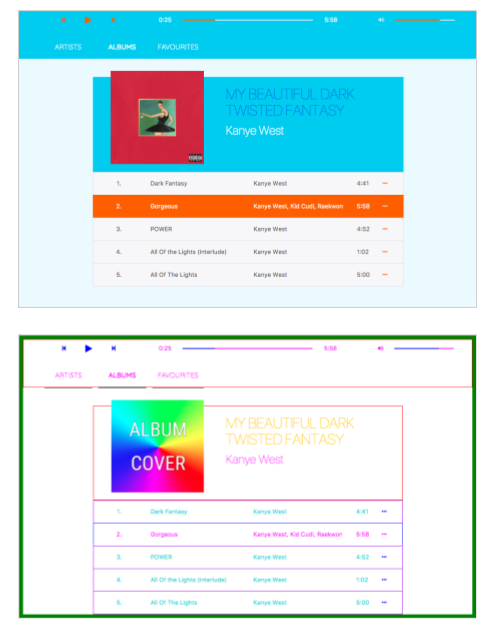
\includegraphics[width=1\textwidth]{img/color_groups.png}
	\caption{Beispiel der Farbgestaltung einer exemplarischen Weboberfläche für Musik-Streaming. (a) Generische Farbgestaltung ohne Anpassung an das Albumcover. (b) Separate Hervorhebung der sechs Color Groups. Elemente einer Color Groups sind jeweils rot dargestellt. (c) Beispiel einer Farbgestaltung mit Anpassung an das Album Cover.}
	\label{fig:colorgroups}
\end{figure*}

Ziel dieser Arbeit ist die automatisierte Bestimmung der Farbwerte von Elementen in Webseiten. Der CSS-Standard zur Beschreibung der Formatierung von HTML-Dokumenten definiert mehr als 10 Eigenschaften zur farblichen Gestaltung, wobei einige spezifisch für bestimmte  HTML-Elemente sind  \citep{css3-color}. In dieser Arbeit werden die Farbeigenschaften von zwei verschiedenen Arten von Oberflächenkomponenten betrachtet:
\begin{enumerate}
	\item \textbf{Texte}: Elemente mit transparentem Hintergrund (\texttt{background-color: transparent}) und definierter Vordergrundfarbe (\texttt{color}). 
\end{enumerate}
\texttt{<h1>}, \texttt{<a>}, etc.) betrachtet. Elemente, die visuell als Blöcke wahrgenommen werden (d.h. die Hintergrundfarbe \texttt{"background-color"} von \texttt{<div>}, \texttt{<button>} etc.) und (2)  Es wird also die Farbbestimmung von \textbf{Blöcken} und \textbf{Texten} fokussiert. Rahmen, Textdekoration und andere färbbare Komponenten werden vernachlässigt.

Üblicherweise werden mehrere Elemente eines HTML-Dokuments auf die gleiche Farbe abgebildet. Beispielsweise können alle Links (Textfarbe) sowie Buttons (Hintergrundfarbe) in Blau dargestellt werden. Im Folgenden wird eine Menge von Elementen einer Webseite mit gleicher Farbabbildung als \textbf{Color Group} $CG$ bezeichnet \citep[siehe auch][]{webpage, patterns}. 

 Die Menge aller Color Groups einer Webseite wird als $CGs$ formalisiert. Es gilt $|CGs| = k$. Eine Webseite mit $k$ Color Groups tritt also mit $k$ Farben in Erscheinung. Abbildung \ref{fig:colorgroups} veranschaulicht dies anhand einer exemplarischen Webseite für Musik-Streaming. (a) zeigt ein generisches Farbdesign, während (b) die sechs Color Groups separat hervorhebt.

Webdesigner verkleinern Suchraum zur Identifizierung geeigneter Farben für die Color Groups durch die Zusammenstellung einer sogenannten \textbf{Farbpalette} \citep{webpage, webdesign, webx0}. Dabei handelt es sich um eine Farbmenge $P = \{c_1, c_2, \ldots, c_n\}$ mit $n$ Farben, wobei jedes $c \in P$ als String von RGB Werten kodiert wird. Formal ist damit das Ziel dieser Arbeit die Ermittlung einer Abbildung $CGs \to P$. Die Abbildung muss injektiv sein, d.h. nicht jede Farbe der Farbpalette $P$ muss verwendet werden, jedoch dürfen mehrere Color Groups nicht gleich gefärbt werden. Es gilt $k \leq n$.

Entscheidendes Kriterium für die Zuordnung ist eine funktionale Gestaltung der Webseite. Im Rahmen dieser Arbeit wird hierunter eine Farbgestaltung verstanden, die Lesbarkeit und Benutzerführung gewährleistet. Eine intuitiv widersinnige Färbung ist beispielsweise ein roter Text auf orangem Hintergrund mit grauem Button. Weder ist der Text lesbar, noch wird die Aufmerksamkeit des Nutzers auf das Interaktionselement gelenkt.

Als Besonderheit dieser Arbeit soll die Farbpalette auf einer Bildvorlage basieren. So wird eine Harmonisierung des visuellen Eindrucks einer Weboberfläche und einer darin präsenten Grafik erreicht. Da die gewählte Farbgebung wesentlich für die vermittelte Atmosphäre einer Webseite ist \citep{webdesign}, soll die Anpassung der Farbgebung an ein Motiv dessen Eindruck unterstützen. Da die Farbpalette somit auf den verarbeiteten Daten basiert, ist eine Berechnung zur Laufzeit möglich, wenn ein effizientes Suchverfahren umgesetzt wird. Ein Anwendungsbeispiel hierfür ist die farbliche Anpassung einer Seite für Musikstreaming an das gespielte Albumcover. Abbildung \ref{fig:colorgroups} (c) zeigt hierfür ein Beispiel.

\subsection{Color Palette Estimation}

Die Zusammenstellung einer Farbpalette aus einer Bildvorlage wird von \citet{acopa} als \textbf{Color Palette Estimation} (CPE) bezeichnet und als die Repräsentation eines Bildes mit einer minimalen Menge von Farben beschrieben. \glqq{}Minimal\grqq{} bedeutet nach Auffassung der Autoren, dass redundante Farben reduziert und die seltenen Farben der für die Wahrnehmung wichtigen Objekte erhalten bleiben. Formale Kriterien werden hierfür jedoch nicht geliefert. Abbildung \ref{fig:ladybug} veranschaulicht diese intuitive Definition am Beispiel eines Bildes mit einem Marienkäfer, dessen Sichtbarkeit von der Wahl der Farbpalette abhängt.

\begin{figure}[h]
\centering
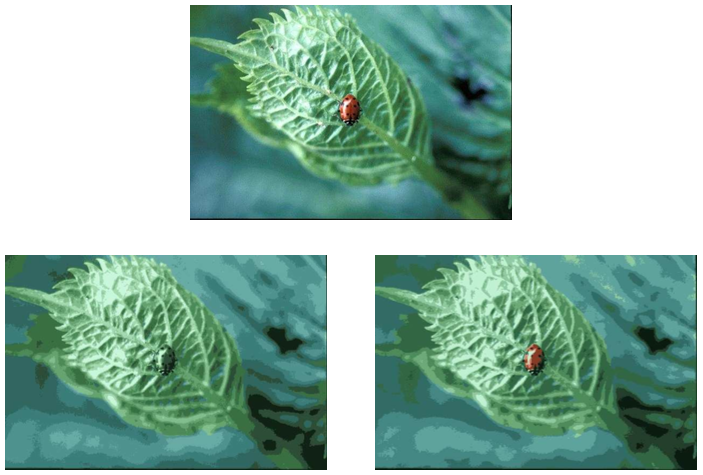
\includegraphics[width=0.48\textwidth]{img/ladybug.png}
\caption{Beispiel für die Einfärbung eines Bildes mit unterschiedlichen Farbpaletten der Größe 12. Oben: Originalbild. Links: Farbpalette ohne rote Farbtöne. Rechts: Farbpalette mit roten Farbtönen, wodurch der Marienkäfer erkennbar ist (Quelle: \citep{acopa})}
\label{fig:ladybug}
\end{figure}

Historisch geht die CPE aus der Farbquantisierung hervor, bei der die Farben von Grafiken aufgrund der damals zu kleinen Kapazität von Grafikpuffern vor deren Anzeige reduziert (Farbreduktion) und dann auf die reduzierte Farbpalette abgebildet werden mussten (Quantisierung) \citep{variance}. Aus diesem Kontext kommt das formale Kriterium der Summe des quadratischen Fehlers, welcher in diesem Anwendungsfall auch als \emph{Recoloring Error} bezeichnet wird \citep{colorthemes}.

Da Grafikpuffer mittlerweile über ausreichend Kapazität verfügen, liegt die Anwendung der CPE in anderen Bereichen wie z.B. der farbbasierten Indizierung von Grafiken in Datenbanken oder der Zusammenstellung von Farbthemen zu Gestaltungszwecken. \citet{colorthemes} zeigen, dass in letzterem Kontext der Recoloring Error keine geeignete Metrik zur Beurteilung der Güte einer Farbpalette in Bezug auf die Bildvorlage ist. Grund sind die menschlichen Wahrnehmungseigenschaften, wobei Bilder auf Komponenten- und nicht auf Pixelebene erfasst werden. Stattdessen werden eine Reihe anderer Metriken vorgestellt, die diesen Umstand berücksichtigen. Die Autoren zeigen zusätzlich empirisch, dass abhängig vom Individuum ein und dieselbe Farbpalette eines Bildes für unterschiedlich repräsentativ gehalten wird. 

Dieser Befund hebt hervor, dass die Güte einer Farbpalette in Bezug auf die Bildvorlage subjektiv ist und vom Anwendungsbezug abhängt. Aus diesem Grund wird für die Beurteilung der zu ermittelnden Farbpalette keine objektive Bewertungsfunktion herangezogen. Stattdessen wird die Zweckmäßigkeit der Farbpalette in Hinblick auf die farbliche Gestaltung von Webseiten fokussiert. Das bedeutet, dass die aus der Bildvorlage hervorgehende Farbpalette eine Teilmenge an Farben beinhalten muss, mit welcher die automatisierte Farbgestaltung einer Webseite lösbar ist. Hierfür müssen Kriterien abgeleitet werden, indem Prinzipien für eine funktionale Gestaltung von Webseiten sowie Farbdefinitionen aus Style Guides analysiert werden. Davon ausgehend wird eine geeigneter Algorithmus zur Bestimmung einer solchen Farbpalette aus einer Bildvorlage ermittelt.

\subsection{Einordnung und Literaturbesprechung}

Die Arbeit ordnet sich in das Gebiet der automatisierten Farbgestaltung (Color Design Automation) ein. In diesem Bereich hat in den letzten Jahren Forschung in verschiedenen Anwendungsbezügen stattgefunden, wobei überwiegend Methoden des maschinellen Lernens zur Problemlösung eingesetzt wurden.

\citet{colorcomp} haben 2011 eine Grundlage für datengetriebene Farbgestaltungssysteme gelegt, indem sie ein Regressionmodell zur Bewertung der Farbkompatibilität von 5 Farben entwickelt haben, d.h. die Bewertung der Farbharmonie von fünf-farbigen Paletten. Hierfür wurde ein Training an den Datenbeständen von Farbpaletten-Communities wie z.B. Adobe Color\footnote{\url{https://color.adobe.com/de/explore/}} durchgeführt. Dabei hat sich unter anderem ergeben, dass die auf geometrischen Strukturen im Farbkreis beruhenden Modelle der klassischen Farbentheorie Farbhamonien nicht zufriedenstellend voraussagen können und in bestimmten Fällen sogar kontraproduktiv sind. Hierzu zählen zum Beispiel die Farbton-Schablonen von \citet{itten} oder \citet{munsell}. Dies ist insofern bemerkenswert, als dass diese Modelle in zahlreichen Unterstützungswerkzeugen zur Farbgestaltung ihre Umsetzung finden. Die Grenzen des trainierten Modells liegen in der Bewertung der Harmonie von Farben mit unterschiedlicher räumlicher Ausprägung \citep{webpage, patterns}. Eine Matlab-Implementierung des Modells zur Überprüfung von Farbharmonien steht öffentlich zum Download bereit \footnote{\url{http://www.dgp.toronto.edu/~donovan/color/}}.

\citet{patterns} haben sich 2013 mit der Lösung einer grundlegenden Form eines Färbungsproblems auseinandergesetzt: Die Kolorierung von Mustern nach dem Prinzip "Malen nach Zahlen". Hierfür wurde ein probabilistisches Modell entwickelt, indem über 8000 von Künstlern entworfene Muster von der Seite \url{http://www.colourlovers.com/} ausgewertet wurden. Die Autoren stellen Kriterienw zur Bestimmung von Hintergrund- und Vordergrundfarben sowie zur Kontrastberechnung vor, die für diese Arbeit genutzt werden können. Zur Lösungssuche wird ein \emph{Factor Graph} genutzt, was ebenfalls ein Ansatz für die vorliegende Arbeit darstellt. Das Modell von \citet{colorcomp} wird als externer Bestandteil des Graphen hinzugefügt, um eine globale Kompatibilität der eingesetzten Farben zu gewährleisten. Eine Anwendung, welche die Autoren vorschlagen, stellt die Umkehrung des Ziels dieser Arbeit dar: Die Anpassung eines Musters an das Farbschema einer Webseite.

\citet{webpage} haben sich 2016 mit der automatisierten Farbgestaltung von Webseiten auseinandergesetzt. Durch die Auswertung von 500 Webseiten wurde ein probabilistisches Modell in Form eines Optimierungsproblem mit mehreren Zielfunktionen entwickelt. Eine der Zielfunktionen gewährleistet ausreichenden Kontrast zwischen den Oberflächenelementen. Eine andere Zielfunktion passt die Farbgestaltung an ein Schlüsselwort an (z.B. \glqq{}Business\grqq{} oder \glqq{}Fresh\grqq{}). Die letzte Zielfunktion wird durch das Modell von \citet{colorcomp} realisiert und gewährleistet Farbharmonie. Die Optimierung wird durch eine lexikographische Strategie umgesetzt, bei welcher in Interaktion mit einem Gestalter die Zielfunktionen nacheinander angewendet werden. Die verwendeten Farbpaletten stammen von der Adobe Color Seite. Als alternatives Anwendungsbeispiel extrahieren die Autoren eine Farbpalette aus einer Grafik und nutzen diese als Grundlage zur Färbung der Webseite. Zur CPE wurde der K-Means Algorithmus verwendet. Im Gegensatz zum Ziel dieser Arbeit erfordert der vorgestellte Prozess jedoch eine Nutzerinteraktion aufgrund der lexikographischen Strategie bei der Optimierung. Somit handelt es sich bei der vorgestellten Lösung um ein Unterstützungswerkzeug und nicht um ein System zur vollautomatisierten Bestimmung einer Farbgestaltung.

\citet{magazines}  haben sich 2013 mit der automatisierten Farbgestaltung von Magazin-Covers auseinandergesetzt. Vergleichbar mit \citep{webpage} wird auch hier die Optimierung des Farbkontrasts, der Farbharmonie und der Farbsemantik verfolgt.  Im Gegensatz zu den bisherigen Lösungen wird hier allerdings mit expliziten Regeln zur Bewertung von Farbharmonien- \citep{itten} und Kontrasten anstatt mit Modellen gearbeitet, die sich aus Trainingsdaten ableiten. Über Flowcharts vermitteln die Autoren Lösungsprozeduren zur Suche geeigneter Schriftfarben und Stellen konkrete Grenzwerte vor, die für diese Arbeit übernommen werden können.

\section{Problemlösungansatz und Systemarchitektur}

Ausgehend von der Literaturbesprechung wird ein Ansatz zur Problemlösung besprochen. Darauf aufbauend wird eine konkrete Architektur des zu implementierenden Systems entwickelt. Anschließend werden für die einzelnen Teilaufgaben der Architektur geeignete Methoden besprochen und ausgewählt.

\subsection{Regelbasierter oder probabilistischer Ansatz}

\citet{webpage} stellen für die automatisierte Farbgestaltung zwei grundlegende Herangehensweisen vor:

\begin{enumerate}
	\item \textbf{Regelbasiert:} Beschreibt quantitative Modelle mit determinstischem Regelwerk. Die Arbeit von \citet{magazines} stellt hierfür ein Beispiel dar. Durch die Analyse von Farbharmonie-Modellen wurden Regeln für die automatisierte Gestaltung von Magazin-Covers abgeleitet.
	\item \textbf{Datengetrieben:} Beschreibt Modelle, welche die Performanz möglicher Lösungen einer automatisierten Farbgestaltung auf Grundlage existierender Beispieldaten vorhersagt.
\end{enumerate}

Die regelbasierten Modelle treffen feste Aussagen im Gegensatz zu probabilistischen Modellen, tendieren jedoch zur zu starken Vereinfachung des Problems und abstrahieren damit vom Anwendungsbezug. Im Gegensatz dazu stützen sich die Modelle des datengetriebenen Ansatzes auf reale Beispiele und tendieren daher zu robusteren Ergebnissen in der Anwendungsdomäne \citep{webpage}.

Da bei den probabilistischen Modellen alle potentiellen Lösungen bewertet und gegeneinander abgewogen werden müssen, sind hohe Laufzeiten möglich. Die bereits entwickelte Lösung von \citet{webpage} zur automatisierten Farbgestaltung von Webseiten benötigt selbst nach einer Optimierung des Suchverfahrens, bei der unwahrscheinliche Lösungen frühzeitig ausgeschlossen werden, 2 Stunden zur Konvergenz. Außerdem ist deren vorgestellter Prozess zur Anpassung der Farbgestaltung einer Webseite an eine Bildvorlage nicht im eigentlichen Sinne automatisiert: Einerseits erfordert die Verwendung des K-Means Algorithmus zur CPE die Eingabe der Farbanzahl (k) vom Gestalter, andererseits erfordert die lexikographische Strategie einen Nutzerinteraktion während des Optimierungsprozess.

Aus diesen Gründen wird sich diese Arbeit auf einen \textbf{regelbasierten} Ansatz \textbf{ohne Nutzerinteraktion} konzentrieren. Auch ohne die Auswertung großer Datenmengen existieren quantitative Modelle, um die Accessibility einer Webseite zur gewährleisten. Beispielsweise geben die \emph{Web Content Accessibility Guidelines} \citep{wcag} quantitative Grenzwerte für die Lesbarkeit von Texten an. Es sind Eigenschaften und Bedingungen zu erarbeiten, die für Farben einzelner Color Groups sowie zwischen diesen gelten sollen. Diese Einschränkungen werden im Folgenden als \textbf{Constraints} bezeichnet. Ein System von Constraints mit endlichem Wertebereich (in diesem Fall $P$) wird als \textbf{Constraint Satisfaction Problem} (CSP) bezeichnet \citep{constraint-programmierung}. \citet{magazines} haben gezeigt, dass eine Lösung eines solchen Constraint-Systems beispielsweise über Faktor-Graphs möglich ist.

\subsection{Layouts}

Nicht jede Webseite hat die gleiche Anzahl Color Groups. Um die Komplexität des Constraint-Systems zu reduzieren, wird die Festlegung der Color Groups einer Webseite aus der Betrachtung entfernt. Dafür wird von einer Webseite als \textbf{Layout} abstrahiert. Für ein Layout wird als konstant angenommen, welche Color Groups mit welcher Semantik existieren. Beispielsweise definiert ein Layout eine Color Group, welche alle Buttons beinhaltet und deren Semantik \emph{Interaktion} ist. Aus Sicht des Constraint-Systems werden keine Farben für einzelnen Buttons, sondern eine Interaktionsfarbe gesucht. Durch das Konzept der Color Groups wird somit von den betreffenden Elementen abstrahiert.

\begin{figure*}
	\centering
	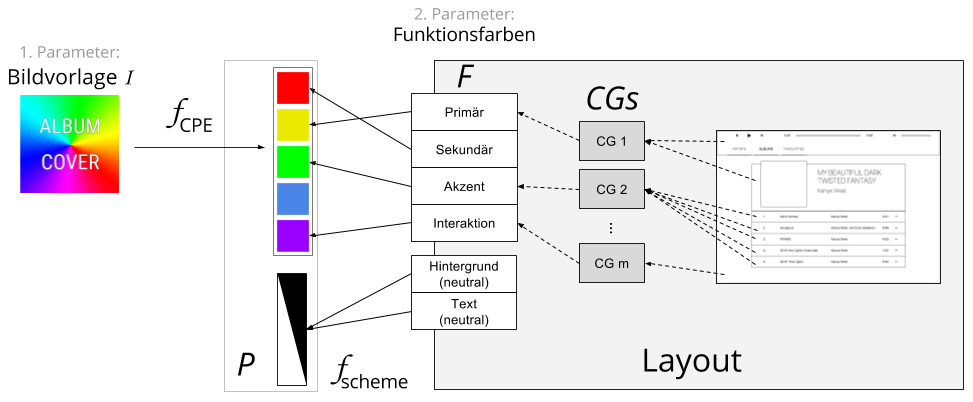
\includegraphics[width=1\textwidth]{img/architecture.png}
	\caption{System-Architektur. Der grau unterlegte Kasten visualisiert den Bereich, für den algorithmische Lösungen gefunden werden müssen. Die Eingabeparameter sind eine Bildvorlage und eine Menge von Color Groups, welche von einem Layout definiert werden. Das System setzt zwei Suchverfahren um, welche mit $f1$ und $f2$ bezeichnet werden. $f1$ ermittelt zuerst eine Farbpalette aus der Bildvorlage (CPE). $f2$ ordnet Colour Groups Farben aus der Palette, in dem ein entsprechendes Constraint System gelöst wird. Nachdem eine Farbabbildung gefunden wurde, wird das kolorierte Layout ausgegeben. }
	\label{fig:architecture}
\end{figure*}

\subsection{Aufteilung der Suchverfahren}

Zur Lösungssuche mit einem regelbasierten Ansatz existieren zwei Herangehensweisen:
\begin{enumerate}
    \item \textbf{Constraints-First}: Setze $n = k$. Hierbei wird die Lösungssuche zum Zeitpunkt der CPE verlagert. Unter Kenntnis der Color Groups ist hier der Suchraum das Histogram der Bildvorlage. Dieser Ansatz wird unter anderem von \citet{colorcomp} verfolgt. Sie verwenden ihr Regressionsmodell zur Bewertung der Farbharmonie, um eine alternative Optimierungsfunktionen zur Suche von $P$ im Farbraum einer Bildvorlage zu formulieren.
    \item \textbf{Constraints-Last}: Setze $k \leq n$. $P$ wird unabhängig vom Layout ermittelt. Der Suchraum beschränkt sich dann auf die Elemente in $P$. Dieser Ansatz wird unter anderem von \citet{documentpalette} bei der automatisierten Farbgestaltung von Dokumenten verfolgt. Nach der Bestimmung einer Farbpalette aus einer Bildvorlage werden sukzessive geeignete Farben aus $P$ ausgewählt. Zuerst wird die Hintergrundfarbe des Dokuments komplementär zum Hintergrund des Bildes gewählt, welche via Bildsegmentierung bestimmt wird. Daraufhin wird die Textfarbe unter Beachtung des Kontrastes aus $P$ gewählt.
\end{enumerate}

Für diese Arbeit wird die Herangehensweise \textbf{Constraints-Last} bevorzugt. Sie beinhaltet die Aufteilung des Problems in zwei getrennte Suchverfahren: Ein Suchverfahren für die Bestimmung von $P$ und ein Suchverfahren zur Bestimmung der Abbildung $CGs \to P$. Dadurch wird eine Wiederverwendung einmal bestimmter Farbpaletten für verschiedene Layouts ermöglicht. Für die Arbeit bedeutet dies, dass eine Problemlösung anhand eines exemplarischen Layouts mit bestimmten Color Groups gezeigt wird, eine Übertragung auf andere Layouts jedoch möglich ist. Schlussendlich ermöglicht ein Cashing bereits berechneter Farbpaletten das Einsatzpotential der automatisierten Farbgestaltung zur Laufzeit, da nur noch eines des Suchverfahren durchgeführt werden muss.

Selbst unter den gegebenen Einschränkung des Suchraums durch die vorgeschaltete Ermittlung einer Farbpalette ist die Menge potentieller Lösungen mit $\binom{n}{k} k!$ nach wie vor groß. Als Beispiel sei ein Layout mit 5 Colorgroups (z.B. Text, Texthintergrund, Buttons, Navigations-Hintergrundfarbe und Footer-Hintergrundfarbe) sowie eine Farbpalette mit 10 Farbe gegeben. Das bedeutet $|CGs| = k = 5$ und $|P| = n = 10$, wodurch sich $\binom{10}{5} 5! = 30.240$ mögliche Kombinationen ergeben. Es ist ein effektives Suchverfahren zur Ermittlung von $CGs \to P$ zu identifizieren. Der bereits vorgestellte, hierarchische Ansatz von \citet{documentpalette} stellt hierfür eine Inspiration dar, bei welchem entscheidende Farbzuordnungen zuerst getroffen werden und dadurch der Suchraum für folgende Color Groups eingeschränkt wird (z.B. erst Hintergrund, dann Textfarbe).

\subsection*{Zusammenfassung}

Abbildung \ref{fig:architecture} fasst den Ablauf der automatisierten Farbgestaltung einer Webseite zusammen. Das zu entwickelnde System bildet eine Bildvorlage auf eine Farbpalette ab. Das Suchverfahren hierfür wird was als Color Palette Estimation (CPE) bezeichnet. Die entstandene Palette wird zum Suchraum möglicher Farben von Color Groups, welche durch ein Layout definiert werden. Da bei dieser Abbildung der Wertebereich einer Color Group dementsprechend beschränkt ist, handelt es sich um ein Constraint Satisfaction Problem (CSP). Letztendlich wird eine kolorierte Variante des Layouts ausgegeben.

Im Folgenden sind konkrete Verfahren für die beiden Teilprobleme CPE und CSP zu implementieren. Ausgangspunkt hierfür sind Prinzipien für eine funktionale Gestaltung von Webseiten. Diese werden im Folgenden durch Webdesign-Literatur sowie die Analyse von Farbdefinitionen aus Style Guides ermittelt.

\section{Farbgestaltung von Webseiten}
Die Ziele der farblichen Gestaltung im Rahmen dieser Arbeit sind Lesbarkeit und Benutzerführung. Im Folgenden werden Gestaltungsprinzipien für diese beiden Ziele herausgearbeitet und als Grundlage für die weiteren Entscheidungen zur Problemlösung betrachtet.

\subsection{Lesbarkeit}
\label{sec:lesbarkeit}

Eine Auswertung von über 100.000 Webseiten hat ergeben, dass Text fast ausschließlich in Graustufen dargestellt wird \citep{webzeitgeist}. Die populärsten Farben sind Schwarz, Dunkelgrau und Weiß. \citet{webdesign} begründet dies damit, dass Text schlechter lesbar wird, je farbiger er ist. Der Style Guide von Googles Material Design \citep{google} hebt hervor, dass Aufgrund des Simultankontrasts die Verwendung von Grau als Textfarbe bei stark farbigem Hintergrund zu unerwünschten Effekten führt, wie Abbildung \ref{fig:text_color} veranschaulicht. Stattdessen wird in Abhängigkeit von der Luminanz des Hintergrunds die Verwendung von Schwarz bzw. Weiß mit einem Alpha-Wert (Transparenz) empfohlen. Konkret werden folgende Werte genannt:
\begin{enumerate}
	\item Dunkle Schrift: $\text{rgba}(0, 0, 0, 0.87)$
	\item Helle Schrift: $\text{rgba}(255, 255, 255, 1.0)$
\end{enumerate}

\begin{figure}[h]
	\centering
	
\includegraphics[width=0.48\textwidth]{img/text_color.png}
	\caption{Empfohlene Textfarbe bei farbigem Hintergrund. (a) Textfarbe $\text{rgb}(114,114,114)$. Der Text ist aufgrund des Simultankontrasts unangenehmer zu lesen. (b) Textfarbe $\text{rgba}(0, 0, 0, 0.54)$, d.h. Schwarz mit einem Alphawert (Transparenz) von $54\%$. Die Textfarbe ergibt sich zu einer Schattierung der Hintergrundfarbe und vermeidet so den Simultankontrast. (Quelle: \citep{google})}
	\label{fig:text_color}
\end{figure}

Im Folgenden wird die Textfarbe mit Ausnahme von Fällen, in denen die Schrift aus stilistischen Gründen bunt erscheinen soll, auf diese Werte festgelegt. Es ist zu entscheiden, wann die dunkle und wann die helle Textfarbe verwendet wird. Hierfür geben die Web Content Accessibility Guidelines (WCAG) des W3C konkrete Grenzwerte für Kontrastverhältnisse in Abhängigkeit von der Text- und Hintergrundfarbe sowie der Textgröße an. Die Formel lautet zur Berechnung des Kontrastverhältnisses $L_c$ lautet \citep{wcag-contrast}:

\begin{equation}
	\begin{split}
		L_c(c_1, c_2) = \frac{L(c_1) + 0.05}{L(c_2) + 0.05} \;,\\ L(c_1) \geq L(c_2)
	\end{split}
\end{equation}

mit $L_c \in [1, ... , 22]$, wobei $L_c(weiss, schwarz) = 22$ und $c_1 = c_2: \;L_c(c_1, c_2) = 1$. Die Berechnungsvorschrift der normalisierten relativen Luminanz einer Farbe $L$ ist \citep{wcag-rel-luminance} zu entnehmen.
Es gelten zwei verschiedene Grenzwertklassen \citep{wcag}. Die Grenzwertklasse \emph{AA} beschreibt die Minimalanforderung an lesbaren Text:
\begin{equation}
  	AA: L_c(c_1, c_2) \geq
	\begin{cases}
		\begin{split}3.0, \; \text{Schriftgr.} \geq 18pt \lor \\ \geq 14pt \land fett\end{split} \\
		4.5,  \;  \text{sonst}
	\end{cases}
\end{equation}

Die Klasse \emph{AAA} enthält höhere Grenzwerte und beschreibt verstärkte Lesbarkeit:

\begin{equation}
  	AAA: L_c(c_1, c_2) \geq
	\begin{cases}
		\begin{split}4.5, \; \text{Schriftgr.} \geq 18pt \; \lor \\ \geq 14pt \land fett\end{split} \\
		7,  \;  \text{sonst}
	\end{cases}
\end{equation}

\subsection{Benutzerführung}
\label{sec:usability}
Ein adäquater Farbeinsatz ermöglicht die Steuerung von Aufmerksamkeit und unterstützt die Bildung von Zusammenhängen \citep{webdesign}.  Dieses Konzept wird auch als visuelle Hierarchy bezeichnet \citep{visual-hierarchy}, bei welchem die Oberflächenelemente strukturiert und priorisiert werden.
\citet{webdesign} unterteilt folgende Möglichkeiten zur Benutzerführung durch Farbeinsatz:

\begin{itemize}
	\item \textbf{Themengruppen:} Bedeutet die farbliche Kodierung inhaltlich definierter Bereiche. Hierbei handelt es sich um eine vom Gestalter erfundene, subjektive Farbsystemlogik, die kein System, sondern eine Gestaltungsstuktur darstellt, die dem Anwender zu lernen aufgezwungen wird. Dies resultiert automatisch in Buntheit, welche Aufmerksamkeit erregt und somit kontraproduktiv für die Bildung einer visuellen Hierarchie ist. Aus diesen Gründen ist von dieser Variante abzuraten. Abbildung \ref{fig:theme_coding} verdeutlicht dies am Beispiel eines Online-Magazins.
	\item \textbf{Funktionsbereiche:} Bedeutet die farbliche Kodierung von Bereichen entsprechend ihrer Funktion. So sind beispielsweise Navigations-, Inhalts- und Servicebereich farblich differenzierbar. Diese Variante ist zu empfehlen, wenn nicht mehr als drei Farben verwendet werden und die betreffenden Bereiche gleichzeitig und somit im Bezug zueinander sichtbar sind. Abbildung \ref{fig:functional_areas} verdeutlicht dies am Beispiel einer farblichen Abgrenzung von Navigationsbereichen.
	\item \textbf{Funktionen und Zustände:} Bedeutet die farbliche Kodierung von funktionstragenden Elemte oder deren Funktionszustände. Beispielsweise sind anklickbare Elemente (z.B. Links und Buttons) durch eine einheitliche Farbe signalisierbar. Abbildung \ref{fig:functions} zeigt hierfür ein Beispiel Elemente mit destruktiver Funktion, z.B. Buttons zum Löschen oder Abbrechen einer Aktion, können einheitlich rot gefärbt werden. Wurde eine Farbe einmal mit einer Funktion belegt, sollte sie einheitlich verwendet werden. Beispielsweise würde ein nicht-anklickbares, blaues Element in der Oberfläche aus Abbildung \ref{fig:functions} würde verwirren.
\end{itemize}

\begin{figure}[h]
	\centering
	
\includegraphics[width=0.48\textwidth]{img/theme_coding.png}
	\caption{Farbkodierung von Themengruppen am Beispiel von \url{www.smashingmagazine.com/}. Es ist unklar, weshalb die gewählten Farben mit den jeweiligen Bereichen assoziiert werden.}
	\label{fig:theme_coding}
\end{figure}

\begin{figure}[h]
	\centering
	
\includegraphics[width=0.48\textwidth]{img/functional_areas.png}
	\caption{Farbkodierung von Funktionsbereichen am Beispiel von \url{www.leipzig-studieren.de}. Navigationsbereiche (orange) werden zueinander in Bezug gebracht und vom Inhalt (weiß) abgegrenzt.}
	\label{fig:functional_areas}
\end{figure}

\begin{figure}[h]
	\centering
	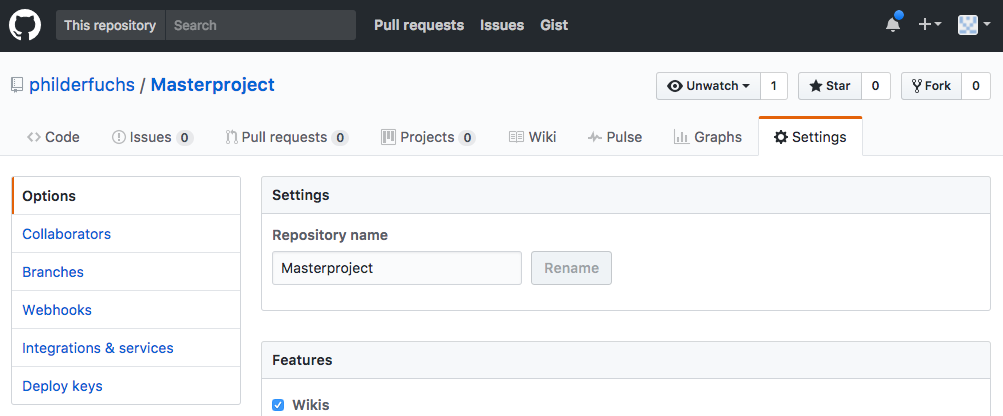
\includegraphics[width=0.48\textwidth]{img/functions.png}
	\caption{Farbkodierung von Funktionen am Beispiel von \url{www.github.com}. Nur anklickbare Elemente sind blau, aktive Elemente werden zusätzlich braun markiert.}
	\label{fig:functions}
\end{figure}

\subsection{Farbfunktionen}
Aus \autoref{sec:usability} geht hervor, dass Elemente entsprechend ihrer Funktion gefärbt werden, nicht aus rein dekorativen Gründen oder zur thematischen Strukturierung. Aus diesen Gründen wird zwischen die Abbildung $CGs \to P$ eine Abstraktionsschicht mit der Bezeichnung \textbf{Farbfunktionen} $F$ geschoben, welche beschreibt, welche Funktion eine Color Group in einer Oberfläche erfüllt. In Anlehnung an \citep{google,  smashing} wird exemplarisch $F = \{\text{Primär}, \text{Sekundär}, text{Interaktion}, \text{Akzent}, \text{Text Hell},\\ \text{Text Dunkel}, \text{Hintergrund}\}$ definiert. Die einzelnen Farbunktionen lauten wie folgt:
\begin{itemize}
	\item \textbf{Primärfarbe:} Wird in Relation zu den anderen Farben am häufigsten eingesetzt und bildet so die farbliche Grundstimmung der Oberfläche \citep{awwwards}.
	\item \textbf{Sekundärfarbe:} Unterstützt die Farbstimmung der Primärfarbe und orientiert sich dementsprechend an deren Farbton. Durch die Wahl einer unbunteren Farbe tritt sie in der visuellen Hierarchie stärker in den Hintergrund \citep{visual-hierarchy}, eignet sich besser als Hintergrund für Fließtext und unterstützt durch den Qualitätskontrast die Wirkung der Primärfarbe \citep{webdesign}.
	\item \textbf{Interaktionsfarbe:} Signalisiert Elemente, mit denen eine Interaktion möglich ist, z.B. klicken. Dies trifft nicht zwangsläufig auf Elemente zu, bei denen der Nutzer eine Interaktionsmöglichkeit aufgrund ihrer Funktionsgruppe bereits erwartet, wie z.B. in der Seitennavigation.
	\item \textbf{Akzent:} Signalisiert Elemente mit hoher Priorität in der visuellen Hierarchie. Dies ist erreichbar durch einen relativ seltenen (Quantitätskontrast, \citep{webdesign}) Einsatz einer bunten \citep{visual-hierarchy} Farbe.
	\item \textbf{Text Hell/Dunkel:} Farbe für Fließtext. Entsprechend \autoref{sec:lesbarkeit} wird hierfür in Abhängigkeit Hintergrund Weiß (Hell) bzw. Schwarz (Dunkel) mit Alpha-Kanal festgelegt.
	\item \textbf{Hintergrund:} Standardfarbe von Blöcken, die keiner der obigen Farbfunktionen entsprechen. Dies betrifft vorwiegend Blöcke mit Fließtext, so dass Textlesbarkeit zu beachten ist. Dementsprechend sind Graustufen zu bevorzugen \citep{webx0}, wobei entsprechend \autoref{sec:lesbarkeit} ein ausreichender Luminanzkontrast zu gewährleisten ist. Darum wird die Hintergrundfarbe analog zur Textfarbe auf Weiß bzw. Schwarz festgelegt.
\end{itemize}

Die hier verwendeten Farbfunktionen sind exemplarisch. Abhängig von den individuellen Ansprüchen einer Webseite ist die Definition weiterer Farbfunktionen denkbar. Bei mobilen Anwendungen ist beispielsweise eine farbliche Differenzierung verschiedener Interaktionsformen sinnvoll (z.B. drücken und wischen).
Die Abbildung zwischen Color Groups und Farbfunktionen wird als die Funktion $S$ definiert und im folgenden als \textbf{Farbschema} definiert. Es gilt: 
\begin{equation}
  S: F \to P
\end{equation}

Diese Definition eines Farbschemas unterscheidet sich von der Verwendung des Begriffs in der Literatur \citep{webdesign}. In dieser ist ein Farbschema eine Charakterisierung einer Farbpalette. Es beschreibt, \emph{wie viele} unterschiedliche Farbtöne eine Farbpalette enthält und in welcher \emph{geometrischen Beziehung} diese zueinander stehender.  Beispielsweise bezeichnet ein \emph{triadisches} Farbschema eine Farbpalette mit drei Farbtönen, die sich in einem Abstand von $120^{\circ}$ zueinander befinden. Genauer wird in  \emph{monochromatische}, \emph{komplementäre (duale)}, \emph{triadische} und \emph{tetraedische} Farbschemen unterschieden, welche Farbpaletten mit einem, zwei, drei oder vier verschiedenen Farbtönen repräsentieren. \citep{underestimated, smashing, google} empfehlen jedoch die Beschränkung auf höchstens 3 Farben im Webdesign, während Graustufen für die Darstellung von Text und Hintergründen dominieren. Dementsprechend werden die Begriffe \textbf{monochrom}, \textbf{dual} und \textbf{triadisch} für die Charakterisierung des Farbschemas als Farbabbildung in dieser Arbeit adaptiert.
    
\autoref{fig:colorschemes} zeigt hierfür Beispiele. Oben wird eine exemplarische \emph{Farbpalette} abgebildet. Die \emph{Farbfunktionen} entsprechen der in diesem Abschnitt definierte Menge $F$. Es ist zu erkennen, dass die Textfarben sowie die Hintergrundfarbe bereits pauschal definiert werden. Damit realisiert jedes Farbschema im Rahmen dieser Arbeit einen \textbf{Bunt-Unbunt-Kontrast}, was nach \citep{webx0} eine allgemeine Empfehlung für Webdesign darstellt. Die Abbildung zeigt weiterhin mögliche Abbildungen zwischen den Farbfunktionen und der Farbpalette unter \emph{Farbschemata}. Ein monochromes Farbschema beschränkt sich auf einen Farbton in verschiedenen Schattierungen. Dadurch wird ein \textbf{Qualitätskontrast} gebildet, welcher die Wirkung der Farbe mit dem höchsten Buntheitswert erhöht. Die inverse Variante des monochromen Schemas veranschaulicht eine Variante mit allgemein dunkler Farbstimmung. Das duale Farbschema besitzt zwei Farbtöne. Da Interaktions- und Akzentfarben weniger häufig auftauchen als die Elemente der Primär- und Sekundärfarben wird hierdurch ein \textbf{Quantitätskontrast} gebildet, der die seltenere Farbe zusätzlich betont und so zur Bildung einer visuellen Hierarchie beiträgt. Das exemplarische tertiäre Farbschema  bildet die Interaktions- und Akzentgruppen auf unterschiedliche Farben ab und differenziert diese so zusätzlich. 

\begin{figure}[h]
	\centering
	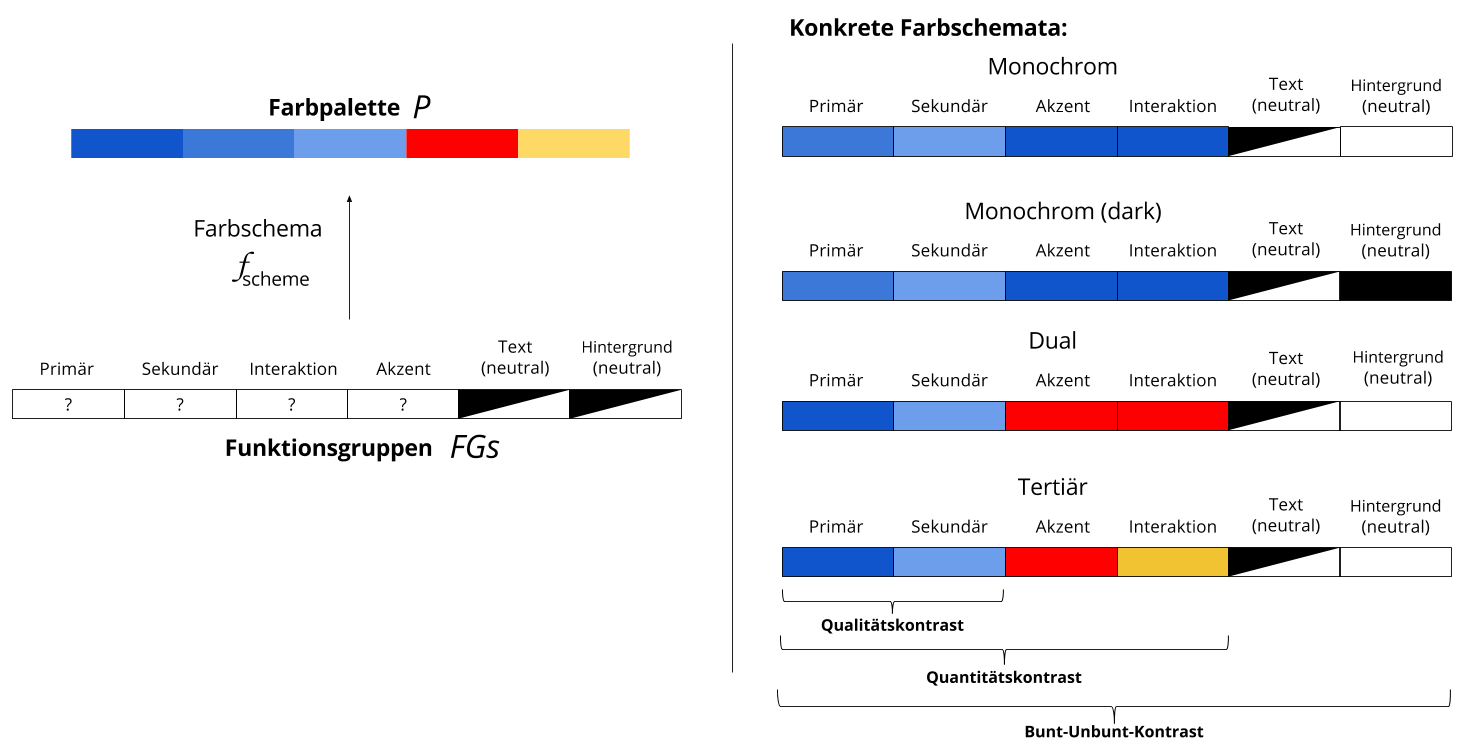
\includegraphics[width=0.48\textwidth]{img/colorschemes.png}
	\caption{Beispiele für monochrome, duale und tertiäre Farbschemata. Der Farbeindruck der Seite wird durch Quantitäts-, Qualitäts- und Bunt-Unbunt-Kontraste bestimmt.}
	\label{fig:colorschemes}
\end{figure}

\subsection*{Zusammenfassung}
Zur Unterstützung der Benutzerführung werden in Webseiten Funktionsbereiche und Elemente mit einheitlicher Funktion bzw. Funktionszustand farblich kodiert. Dementsprechend werden für eine Webseite eine Menge an Farbfunktionen $F$ definiert, wie z.B. die Interaktionsfarbe, welche klickbare Elemente signalisiert. Ein Farbschema $S: F \to P$ ist eine Abbildung der Farbfunktionen auf die Farben einer Palette $P$. Eine Abbildung soll höchstens drei verschiedene Farbtöne enthalten. Für Fließtext sowie dessen Hintergrund werden standardmäßig Graustufen festgelegt. Zur Benutzerführung realisieren Webseiten somit einen Bunt-Unbunt- sowie Quantitätskontrast, welcher das zentrale Gestaltungsmittel des Screendesigns darstellt \citep{webdesign, webx0}.

\section{Algortihmen zur Color Palette Estimation}

Im Folgenden wird eine Algorithmus zur Lösung des Teilproblems der Ermittlung der Farbobermenge $C_s$ gesucht. Hierzu findet eine Betrachtung von Typen vorhandener Algorithmen zur CPE statt. Abschließend wird ein geeigneter Algorithmus ausgewählt

\subsection{Überblick}

Grundlegend sind zwei Ansätze zur CPE zu unterscheiden:
\begin{enumerate}
    \item \textbf{Hisgoram-basiert}: Algorithmen, die nur auf dem Histogramm des Bildes arbeiten und somit die Positionsinformationen der Farben nicht beachten. Es handelt sich (bis auf Ausnahmen) um Clustering-Verfahren, die durch eine Partitionierung des Farbraums Gruppen ähnlicher Farben im Histogramm identifizieren.
    \item \textbf{Bildsegmentierungs-basiert}: Algorithmen, die durch eine Segmentierung des Bildes zunächst zusammenhängende Komponenten identifizieren und für diese dann repräsentative Farben identifizieren.
\end{enumerate}


Bildsegmentierungs-basierte Algorithmen berücksichtigen die menschlichen Wahrnehmungseigenschaften auf Komponentenebene, führen aber durch die zusätzliche Betrachtung der Positionsinformation eine weitere Komplexitätsebene ein \citep{colorthemes}.

\citet{categorization} treffen eine Kategorisierung der Histogramm-basierten Verfahren in \emph{hierarchisch} und \emph{iterativ}. Hierarchisch arbeitende Algorithmen zur CPE werden auch als \emph{Pre-Clustering Verfahren} bezeichnet, da sie vor dem Erreichen der (fest zu wählenden) Farbanzahl $n$ mit mehr bzw. weniger Farben starten. Sie basieren auf der statistischen Analyse der Verteilung der Bildfarben im Farbraum. In diese Kategorie fallen \emph{top-down} bzw. \emph{bottom-up} Clustering-Algorithmen. Zu den Top-Down Verfahren zählen die in der Vergangenheit populären Raumunterteilungs-Algorithmen wie z.B. Mediancut \citep{mediancut} oder Octree\citep{octree}. Sie Zerteilen den Farbraum sukzessiv in disjunkte Teilräume und unterstellen den Clustern dabei eine Würfelform. Ergebnis der Verarbeitung ist ein Dendogram, wobei die Blätter die Farben Farbpalette repräsentieren. Ein Schnitt des Dendograms entspricht einer Partitionierung des Raums, welche jedoch auch direkt durch die iterativ arbeitenden Algorithmen erreichbar ist \citep{acopa}. Diese Verfahren werden darum auch als \emph{partitionierend} \citep{acopa} oder auch \emph{Post-Clustering} \citep{categorization} bezeichnet. Sie starten bereits mit der erforderlichen Anzahl Farben $n$ und verbessern diese iterativ. Einige Methoden dieser Klasse verwenden den quadratischen Fehler, wie z.B. K-Means \citep{kmeans, kmeanshsi} oder Fuzzy C-Means \citep{fuccycmeans}. Andere analysieren das Histogramm auf dichte bzw. weniger dichte Regionen, wie z.B. Mean-Shift \citep{meanshift}. Eine detailliertere Vorstellung von Algorithmen zur CPE bietet \citep{categorization2}.

\begin{figure}[h]
\centering
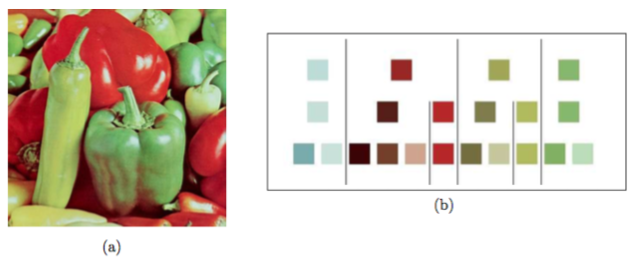
\includegraphics[width=0.48\textwidth]{img/peppers.png}
\caption{CPE Ergebnis von ACoPa. (a) Originalbild "Peppers" (b) Hierarchische Farbpalette. Die unterste Ebene zeigt die finalen Farben. (Quelle: \citep{acopa})}
\label{fig:peppers}
\end{figure}

\citet{acopa} kritisieren an den bisherigen Algorithmen, dass die Anzahl gesuchten Farben $n$ zuvor bekannt sein muss, dass die Ergebnisse abhängig von der Initialisierung sind und dass Farben kleiner Bilddetails im Sinne der Definition in Abschnitt \ref{sec:modellierung} nur unzureichend repräsentiert werden, wie im Paper experimentell nachgewiesen wird. Aus diesem Grund stellen sie den \textbf{Automatic Color Palette (ACoPa)} Algorithmus vor, welcher durch die Analyse von Spitzen des Histogramms im HSI Raums eine Farbpalette erstellt und dabei deren Größe selbstständig bestimmt. Der Algorithmus ermittelt dabei zunächst die grundlegenden Farbtöne (Hue) des Bildes und schlüsselt diese daraufhin sukzessive nach deren Sättigungen (Saturation) und Schattierungen (Intensity) auf. Abbildung \ref{fig:peppers} veranschaulicht exemplarisch die hierarchische Arbeitsweise, bei der in jeder Ebene zusätzliche Sättigungen und Schattierungen der enthaltenen roten und grünen Farbtöne gebildet werden.

\subsection*{Zusammenfassung und Wahl des Algorithmus zur CPE}

Der Algorithmus zur CPE soll eine Obermenge $C_s$ von Farben bilden, aus welcher im einem nachfolgenden Schritt eine Teilmenge von Farben $C$ entsprechend ihrer Eignung für bestimmte Oberflächenelemente ausgewählt werden. Analog dazu werden Farbpaletten in Styleguides als Obermenge von Farben beschrieben, aus welcher der Designer eine Untermenge von Farben für die konkrete Oberfläche auswählt. Bestimmte Styleguides erweitern dabei das Farbpalettenkonzept um Color Swatches, bei welchen Farbtöne in zusätzliche Schattierungen aufgefächert werden. Dadurch hat der der Designer eine größere Flexibilität beim Einsatz der Farbpalette.

Aus diesen Gründen wird der ACoPa Algorithmus von \citet{acopa} zur CPE gewählt.Da er Farbwerte automatisch in verschiedenen Sättigungen und Schattierungen ermittelt, imitiert er die Farbdefinition in Form von Color Swatches in Styleguides. Durch seine parameterfreie Arbeitsweise ermittelt er selbstständig die Anzahl repräsentativer Farben im Bild. Dadurch wird automatisch die erforderliche Obermenge zur Bildung der finalen Farbpalette bereitgestellt, wenn das Bild ausreichend viele Farben enthält. Das erzwingen eines großen Farbpalette mit anderen Clusteringverfahren, z.B. über einen pauschal großen K Parameter bei K-Means, führt hingegen unter Umständen zu einer Partitionierung des Farbraums, die nicht der Clusterstruktur des Histogramms entspricht.

\section{ACoPa}

Im Folgenden wird die grundlegende Arbeitsweise des ACoPa Algorithmus nach \citet{acopa} vorgestellt. Dabei werden die Herausforderungen, die bei der Implementierung aufgetreten sind, besprochen. Abschließend werden exemplarisch Anwendungsergebnisse präsentiert.

\subsection{Konvertierung in den HSI-Raum}

\begin{figure*}
\centering
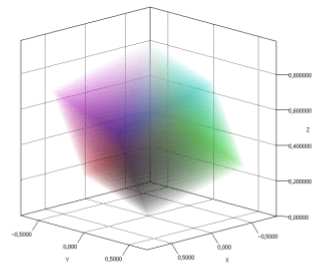
\includegraphics[width=1\textwidth]{img/hsi_conversion.png}
\caption{Gegenüberstellung von RGB zu HSI-Umrechungsergebnisse. (a.) Referenz-HSI Raum. (b.) Umrechnung nach \citep{acopa}. (c.) Umrechnung nach \citep{colorimage}.}
\label{fig:hsi_conversion}
\end{figure*}

Zunächst wird das Histogram in den HSI Farbraum $\{(h, s, i) \ | \ 0 \leq h < 360 \wedge 0 \leq s, i \leq 1\}$ übertragen. Die Intensität eines Farbtons wird dabei in Polarkoordinaten via $h$ und $s$ angegeben, während die maximal mögliche Sättigung wiederum von der Intensität $i$ abhängt. Zur Konvertierung vom RGB in HSI Raum wurden verschiedene Umrechnungsvorschriften erprobt. Die Umrechnung gemäß der ACoPa-Autoren lautet:

\begin{equation}
\begin{split}
I = \frac{R+G+B}{3} \\
S = \sqrt{(R-I)^2 + (G-I)^2 + (B-I)^2} \\  
H = \arccos{(\frac{(G-I)-(B-I)}{S\sqrt{2}})}
\end{split}
\label{eq:hsi_acopa}
\end{equation}

Die Umrechnung gemäß eines Lehrbuchs für Farbbild-Verarbeitung \citep{colorimage} lautet hingegen:

\begin{equation}
\begin{split}
I = \frac{R+G+B}{3} \\
S = 1 - \frac{\min{(R, G, B)}}{I} \\ 
H = \arccos{(\frac{\frac{1}{2}((R-G)+(R-B))}{\sqrt{(R-G)^2+(R-B)(G-B))}})}
\end{split}
\label{eq:hsi_colorimage}
\end{equation}

Abbildung \ref{fig:hsi_conversion} stellt die Umrechnungsergebnisse dem Referenz HSI Raum (R) gegenüber. Keine der Umrechnungsvorschriften führt zu einem Doppelkegel. Weder Formel \ref{eq:hsi_acopa} noch Formel \ref{eq:hsi_colorimage} projiziert die Farben mit 100\% Sättigung ($s = 1$) in eine Ebene. Formel \ref{eq:hsi_acopa} führt lediglich zu einer Drehung und Stauchung des RGB-Würfels, Formel \ref{eq:hsi_colorimage} führt zu einem nach unten geöffneten Kegel. Da schlussendlich keine Formel gefunden werden konnte, die zu einem korrekten Doppelkegel führt, wurde die Berechnung mit Formel \ref{eq:hsi_acopa} fortgeführt.

\subsection{Histogramm-Segmentierung}

Die Samples des Ausgangsbildes werden entlang der Hue-Werte sortiert. Das 1-dimensionale Hue-Histogram $h=(h_i)_{i = 1 \ldots b}$ mit b-Bins wird gebildet. Gesucht wird nun eine Sequenz $s = (s_i)_{i = 1 \ldots k}$ mit $1 = s_0 < s_1 < \ldots < s_k = b$, welche eine Segmentierung des Histograms darstellt. Das Intervall $[{s_i}, s_{i+1}]$ wird als Segment bezeichnet. Ziel ist, dass das Histogramm in den Bereichen $[h_{s_i}, \ldots,  h_{s_{i+1}}]$, eine \glqq annähernd unimodale Verteilung aufweist\grqq \citep{acopa}. Abbildung \ref{fig:unimodal} zeigt das Prinzip an verschiedenen Beispielen.

\begin{figure}[h]
\centering
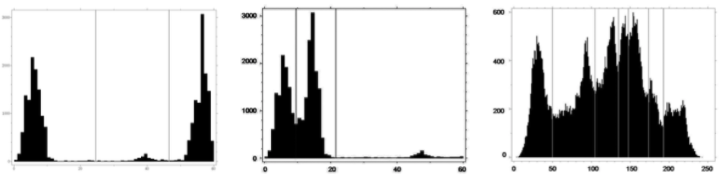
\includegraphics[width=0.48\textwidth]{img/unimodal.png}
\caption{Beispiele der Segmentierung eines Histograms in unimodale Abschnitte. (Quelle: \citep{acopa})}
\label{fig:unimodal}
\end{figure}

Das Histogramm ist offensichtlich in jedem Segment unimodal, wenn $s$ mit den Minima des Histograms initialisiert wird. Es wird nun versucht, Elemente aus $s$ zu entfernen, indem für $\forall i = 1 .. k$ überprüft wird, ob $h$ im Intervall $[h_{s_{i-1}}, \ldots,  h_{s_{i+1}}]$ die \glqq unimodale Hypothese\grqq  erfüllt. Anschaulich bedeutet das die Verschmelzung benachbarter Segmente, so dass das neu entstandene Segment nach wie vor \glqq annähernd unimodal ist\grqq. Hierfür stellen die Autoren in einer separaten Veröffentlichung \citep{ftc} einen parameterfreien statistischen Test vor, der $h$ im betrachteten Intervall mit einem Referenz-Histogramm $h^r$ vergleicht. $h^r$ ist in $[h^r_{s_{i-1}}, \ldots,  h^r_{s_{i+1}}]$ zunächst streng monoton wachsend und danach streng monoton fallend und damit in jedem Fall unimodal. Das Referenz-Histogramm wird aus dem Original-Histogramm $h$ durch Anwendung des Grenander-Operators gebildet. Die komplexen Details hierzu sind \citep{acopa, ftc} zu entnehmen. Da der parameterfreie Test verhältnismäßig aufwändig ist, wird in der eigenen Implementierung auf einen simplen T-Test zurückgegriffen. Dieser liefert ebenfalls befriedigende Ergebnisse, ist aber abhängig vom gewählten Signifikanzniveau.

Das Verfahren zur Histogramm-Segmentierung wird in \citep{ftc} als \textbf{Fine-to-Coarse (FTC) Segmentation Algorithm} zusammengefasst. Zunächst wird $s$ mit allen Minima des Histogramms initialisiert. Daraufhin werden so lange benachbarte Segmente durch Überprüfung der unimodalen Hypothese verschmolzen, bis keine Verschmelzung mehr möglich ist. Die Repräsentanten eines Segments werden durch Mittelung der Samples gebildet, die zum jeweiligen Segment gehören. Abbildung \ref{fig:h_segmentation} zeigt dies an einem Beispiel.

\begin{figure}[h]
\centering
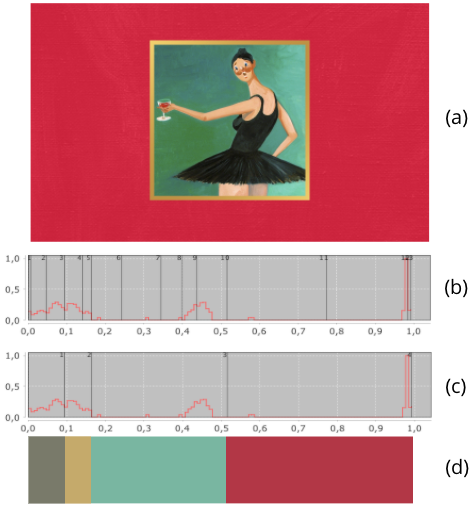
\includegraphics[width=0.48\textwidth]{img/h_segmentation.png}
\caption{Beispiel für eine Segmentierung des Hue-Histogramms. (a) Ausgangsbild, ein Albumcover  von Kanye West. (b) Hue-Histogram (normalisiert), mit allen Minima als initiale Segmentierung. (c) Segmentierung nach Anwendung des FTC Algorithmus. (d) Farbmittelpunkte entsprechend der Samples der jeweiligen Segmente.}
\label{fig:h_segmentation}
\end{figure}

\subsection{Bildung der hierarchischen Farbpalette}

Der ACoPa Algorithmus besteht aus einer hierarchischen Anwendung der Histogram-Segmentierung. Dabei wird zuerst der $h$-, danach der $s$- und abschließend der $i$- Kanal segmentiert. Dabei werden in jedem Schritt die Samples der entstandenen Segmente separiert und die Histogramme der nächsten Ebene getrennt berechnet. Das Ergebnis ist eine hierarchische Farbpalette. Abbildung \ref{fig:palette} zeigt dies am Beispiel der Covers aus Abbildung \ref{fig:h_segmentation}. Auf oberster Ebene (h) wurden die grundsätzlichen Farbtöne des Bildes identifiziert. Auf der zweiten Ebene werden die Farbtöne jeweils in unterschiedliche Sättigungen aufgeteilt, wenn nötig. Auf der dritten Ebene (i) werden von den Sättigungen zusätzlich Helligkeitsabstufungen gebildet.

Die letzte Ebene (i) bildet die Obermenge der Farben $C_s$ für die weitere Verarbeitung. \citet{acopa} empfehlen zusätzlich, die erhaltenen Farben als Startpunkte für den K-Means Algorithmus zu verwenden. Abbildung \ref{fig:palette} (b) zeigt, wie sich die Farben durch K-Means geändert haben. Es ist zu einem späteren Zeitpunkt zu entschieden, welche der beiden Paletten für die weitere Verarbeitung geeigneter ist.

\begin{figure}[h]
\centering
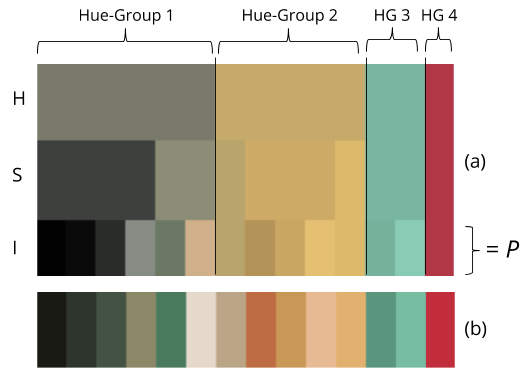
\includegraphics[width=0.48\textwidth]{img/palette.png}
\caption{(a) Hierarchische Farbpalette des Covers aus Abbildung \ref{fig:h_segmentation}. (b) Farbpalette nach Anwendung von K-Means.}
\label{fig:palette}
\end{figure}

\section{Ausblick}

Als nächstes sind die Eigenschaften und Bedingungen der Farben zu ermitteln, die auf der Weboberfläche zum Einsatz kommen sollen. Die Anforderungen müssen in Constraints übersetzt werden. Daraufhin ist ein Algorithmus auszuwählen und zu implementieren, der aus der Farbpalette, die durch ACoPa ermittelt wurde, die passenden Farben herausfiltert. Abschließend werden die Ergebnisse an einer prototypischen Weboberfläche demonstriert.

\bibliographystyle{plainnat}
\footnotesize{\bibliography{references}}

\end{document}
